\documentclass{article} % For LaTeX2e
\usepackage{iclr2025_conference,times}

\usepackage{hyperref}
\usepackage{url}
\usepackage{graphicx}
\usepackage{booktabs}
\usepackage{subcaption}
\usepackage{amsmath}
\usepackage{amssymb}

\title{Deep Learning for Symbolic Music Generation:\\
LSTM Autoencoders, VAEs, and Transformers on MAESTRO}

\author{Safwan Usaid Lubdhak \quad Maidul Islam Moon \quad Random 3rd Person \\
Department of Computer Science and Engineering \\
\texttt{\{lubdhak, moon, random\}@university.edu}
}

\newcommand{\fix}{\marginpar{FIX}}
\newcommand{\new}{\marginpar{NEW}}

\iclrfinalcopy
\begin{document}

\maketitle

\begin{abstract}
We study three deep learning architectures for symbolic music generation using the MAESTRO dataset \citep{Hawthorne2019EnablingFP} (57 MB MIDI-only package): an LSTM Autoencoder, a Variational Autoencoder, and a decoder-only GPT-style Transformer. Each model is evaluated on reconstruction quality, generative diversity, and output structure. The Transformer (Task~3) achieves a final cross-entropy loss of 1.85 and perplexity of 6.36 after 40 epochs, with moderate genre-conditioning capability. Results are reported against random and Markov-chain baselines across pitch histogram overlap, rhythm diversity, and repetition ratio.
\end{abstract}

%-----------------------------------------------------------------------
\section{Exploratory Data Analysis}
%-----------------------------------------------------------------------

We worked exclusively with the 57~MB MIDI-only package of the MAESTRO~v3.0.0 dataset \citep{Hawthorne2019EnablingFP}, which provides 1,276 piano performances with predefined train/validation/test splits in a CSV metadata file. No custom re-splitting was performed.

Figure~\ref{fig:eda} shows our two primary EDA plots.
The duration histogram (Figure~\ref{fig:eda_duration}) shows that most pieces fall in the 3--7~minute range with a long right tail extending to $\sim$30~minutes.
The pitch distribution histogram (Figure~\ref{fig:eda_pitch}) shows that middle-register notes (MIDI pitches 48--72, roughly C3--C5) are the most active, with sparser activity in the extreme low and high registers. This sparsity motivated the use of a class-weighted loss during training.

\begin{figure}[h]
\centering
\begin{subfigure}{0.47\textwidth}
  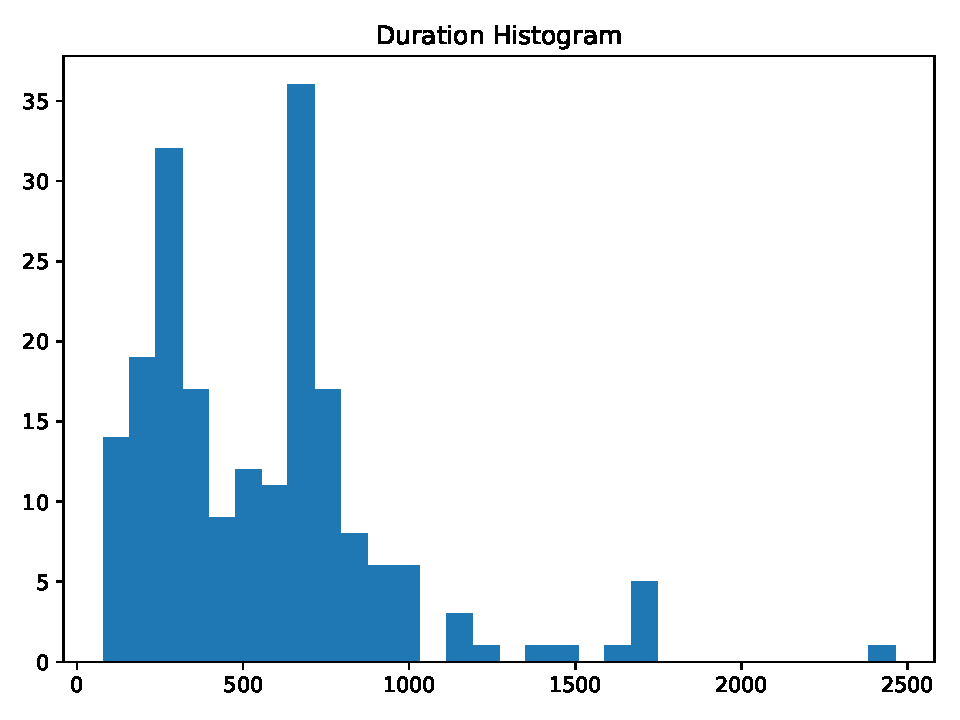
\includegraphics[width=\linewidth]{architecture_diagrams/eda_duration_hist.pdf}
  \caption{Piece duration distribution across the MAESTRO dataset.}
  \label{fig:eda_duration}
\end{subfigure}\hfill
\begin{subfigure}{0.47\textwidth}
  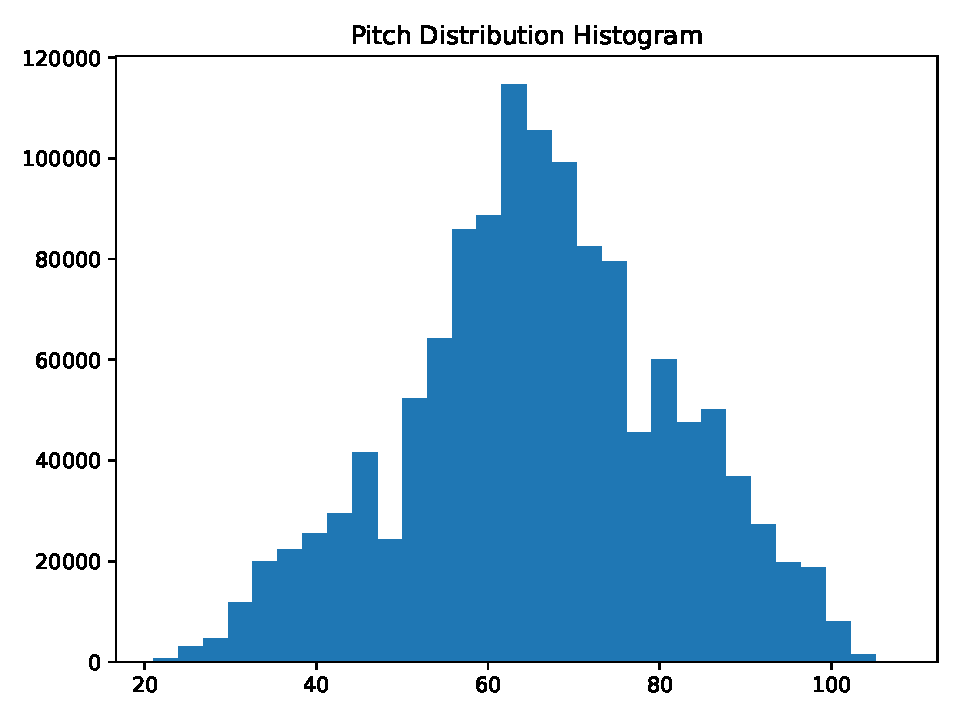
\includegraphics[width=\linewidth]{architecture_diagrams/eda_pitch_hist.pdf}
  \caption{Per-pitch note frequency across a sample of MIDI files.}
  \label{fig:eda_pitch}
\end{subfigure}
\caption{Exploratory Data Analysis. Piano rolls are 88-dimensional binary vectors sampled at a fixed quantisation resolution.}
\label{fig:eda}
\end{figure}

%-----------------------------------------------------------------------
\section{Model Architectures and Implementation}
%-----------------------------------------------------------------------

All models take fixed-length piano-roll segments of shape $T \times 88$, where $T = 128$ time steps and 88 is the MIDI pitch range. Inputs are binary matrices (1 = note active, 0 = note off).

\subsection{Baselines}

\textbf{Random generator.} Notes are sampled i.i.d.\ from a Bernoulli distribution fitted to dataset pitch frequencies.

\textbf{Markov chain.} A first-order Markov model over pitch is estimated from the training set. The row-normalised transition matrix is used for ancestral sampling.

\subsection{Task 1 --- LSTM Autoencoder}

The encoder is a 2-layer LSTM \citep{Hochreiter1997LongSM} ($d_\text{hidden}{=}256$, dropout~$p{=}0.2$) that processes the full segment and projects the final hidden state through a linear layer to a latent code $z \in \mathbb{R}^{64}$:

\[
  z = W_e \, h_T^{(L)}, \quad h_T^{(L)} \in \mathbb{R}^{256}
\]

The decoder is a symmetric 2-layer LSTM that repeats $z$ across all $T$ steps and projects each output to 88-dimensional logits:

\[
  \hat{x}_t = W_d \, h_t^{\text{dec}}, \quad t = 1,\ldots,T
\]

Piano rolls are sparse (under 5\% of cells active), so plain BCE collapses to predicting all zeros. We use \texttt{BCEWithLogitsLoss} with a positive-class weight $w^+$ loaded from \texttt{pos\_weight.txt} (default $w^+ = 20$):

\[
  \mathcal{L}_{\text{AE}} = -\frac{1}{T{\cdot}88}\sum_{t,p}\Bigl[w^+ x_{t,p}\log\sigma(\hat{x}_{t,p}) + (1-x_{t,p})\log(1-\sigma(\hat{x}_{t,p}))\Bigr]
\]

Training used Adam \citep{Kingma2014AdamAM} ($\eta=10^{-3}$, batch size~32) for 40 epochs with gradient clipping at 1.0.

\subsection{Task 2 --- Variational Autoencoder \citep{Kingma2013AutoEncodingVB}}

The VAE uses the same encoder/decoder as Task~1 but replaces the deterministic bottleneck with a stochastic one. Two linear heads map the encoder hidden state to a mean $\mu$ and log-variance $\log\sigma^2$, both in $\mathbb{R}^{64}$:

\[
  \mu = W_\mu h_T^{(L)}, \qquad \log\sigma^2 = W_\sigma h_T^{(L)}
\]

A latent sample is drawn via the reparameterisation trick:

\[
  z = \mu + \varepsilon \odot \sigma, \quad \varepsilon \sim \mathcal{N}(0, I)
\]

The training objective is the negative ELBO:

\[
  \mathcal{L}_{\text{VAE}} = \underbrace{\mathcal{L}_{\text{recon}}}_{\text{BCE sum}} + \beta \underbrace{D_{\mathrm{KL}}\!\left(\mathcal{N}(\mu,\sigma^2)\,\|\,\mathcal{N}(0,I)\right)}_{\displaystyle -\frac{1}{2}\sum_j(1+\log\sigma^2_j - \mu_j^2 - \sigma^2_j)}
\]

To prevent posterior collapse, we used KL annealing \citep{Bowman2015GeneratingSF}: $\beta$ increases linearly from 0 to 1 over the first 10 epochs, then stays at $\beta{=}1$.

\subsection{Task 3 --- GPT-style Transformer}

We implemented \texttt{GPTMusic}, a decoder-only Transformer \citep{Vaswani2017AttentionIA, Huang2018MusicTG} trained autoregressively on tokenised pitch sequences. Architecture details:

\begin{itemize}
  \item \textbf{Token embedding}: $E_\text{tok} \in \mathbb{R}^{V \times 256}$, where $V$ is the vocabulary size.
  \item \textbf{Positional embedding}: learned $E_\text{pos} \in \mathbb{R}^{1024 \times 256}$.
  \item \textbf{Genre embedding}: learnable $E_\text{genre} \in \mathbb{R}^{G \times 256}$, broadcast-added to every position for genre conditioning.
  \item \textbf{Transformer}: 4 decoder layers, 8 heads, FFN width 1024, causal mask via \texttt{generate\_square\_subsequent\_mask}.
  \item \textbf{Output projection}: linear to vocabulary logits.
\end{itemize}

The model is trained to minimise:

\[
  \mathcal{L}_{\text{Trans}} = -\frac{1}{T}\sum_{t=1}^{T} \log \Pr(x_t \mid x_{<t}, g)
\]

%-----------------------------------------------------------------------
\section{Training Results and Loss Curves}
%-----------------------------------------------------------------------

All models were trained on the predefined MAESTRO training split using CUDA. Reported values are at epoch~40. Loss curves use a solid line for training and a dashed line for validation.

\subsection{Task 1 --- Autoencoder Loss}

Figure~\ref{fig:task1_loss} shows the weighted BCE loss. Training loss started at 1.087 (epoch~1) and reached 0.378 at epoch~40. Validation loss ended at 0.431.

\begin{figure}[h]
\centering
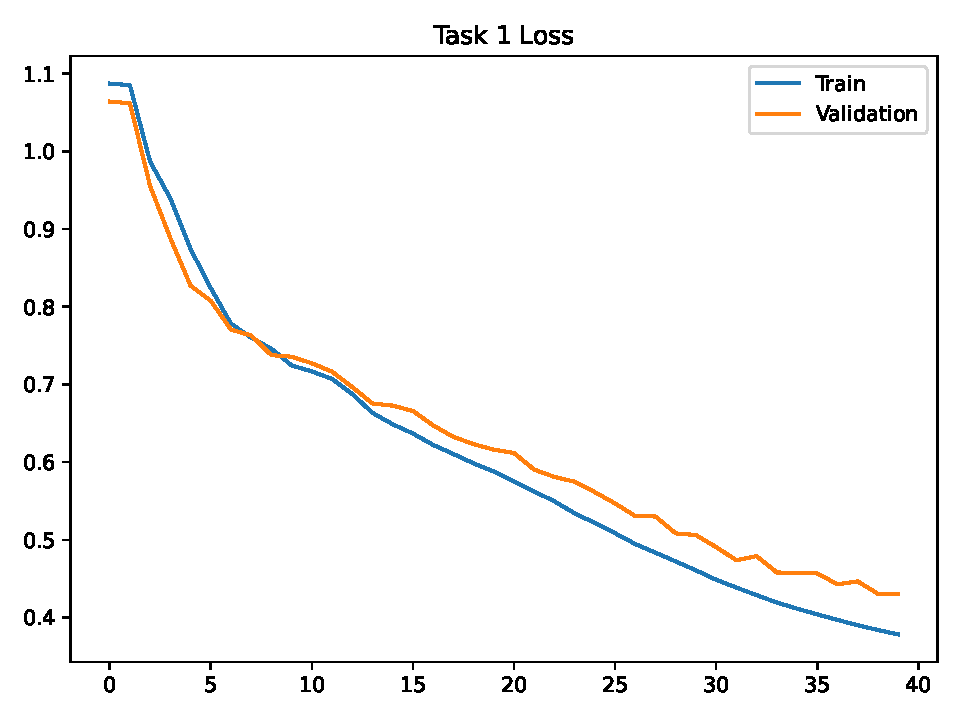
\includegraphics[width=0.60\textwidth]{architecture_diagrams/task1_loss.pdf}
\caption{Task~1: training (solid) vs.\ validation (dashed) BCE loss over 40 epochs.}
\label{fig:task1_loss}
\end{figure}

\subsection{Task 2 --- VAE Loss Components}

Figure~\ref{fig:task2_loss} shows reconstruction and KL loss separately. Reconstruction loss decreased from 11,258 to 3,110 over 40 epochs. KL divergence rose from 66.8 at epoch~1 ($\beta{=}0.1$) to 189.0 once $\beta{=}1.0$ at epoch~10, then plateaued.

\begin{figure}[h]
\centering
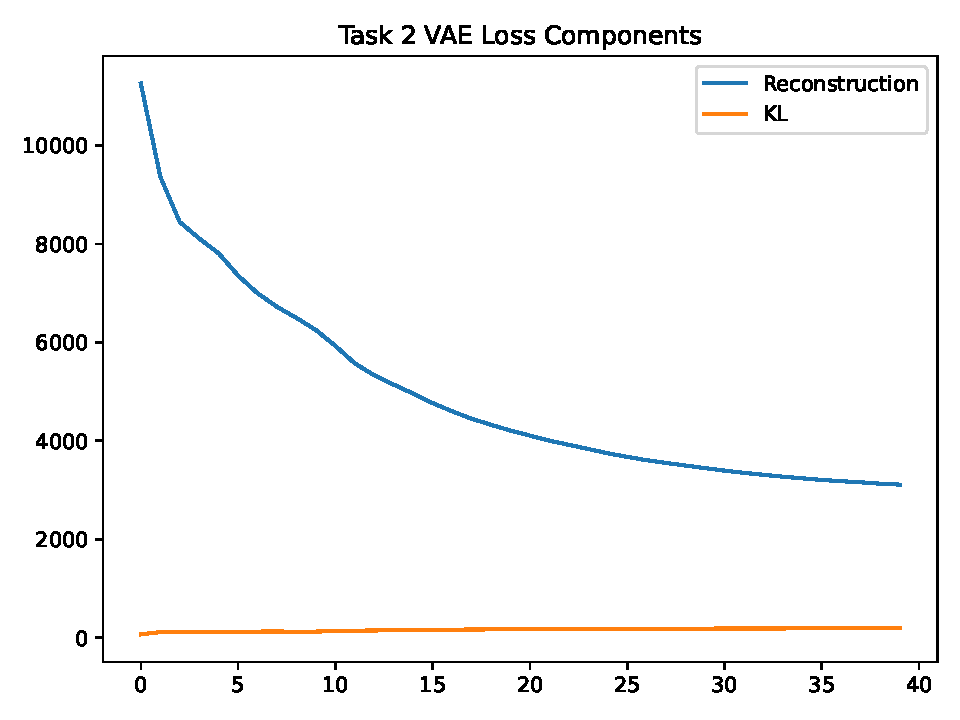
\includegraphics[width=0.60\textwidth]{architecture_diagrams/task2_vae_losses.pdf}
\caption{Task~2 VAE: reconstruction loss and KL divergence over 40 epochs. KL warmup: epochs~1--10 ($\beta$: 0.1$\to$1.0).}
\label{fig:task2_loss}
\end{figure}

\subsection{Task 3 --- Transformer Perplexity}

Figure~\ref{fig:task3_ppl} shows perplexity ($= e^{\mathcal{L}}$) over training. It started at 49.30 (epoch~1) and decreased to 6.36 at epoch~40.

\begin{figure}[h]
\centering
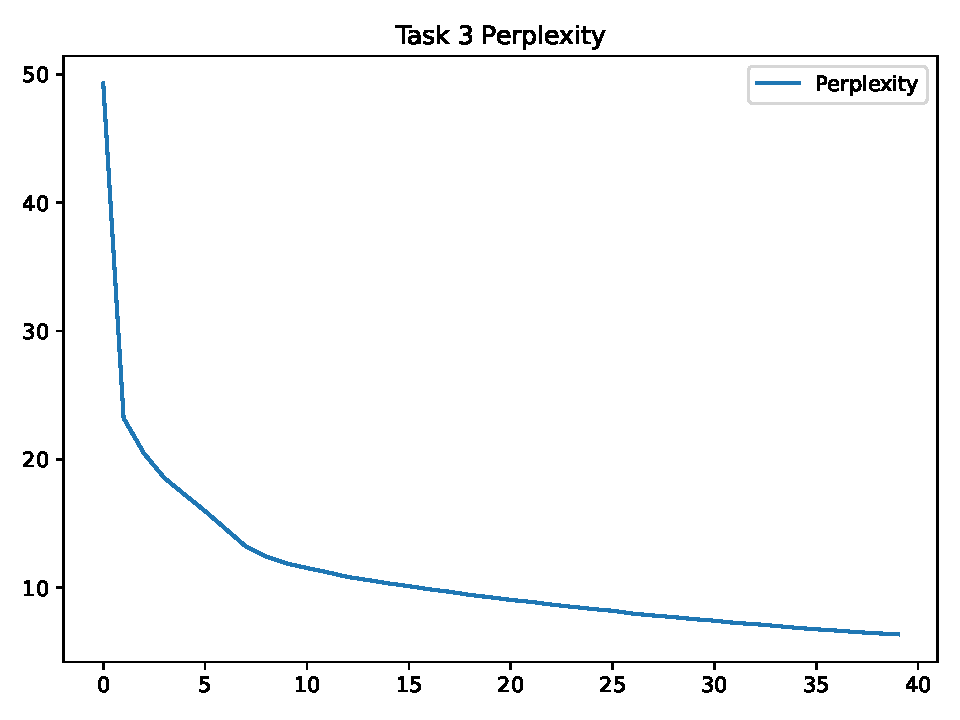
\includegraphics[width=0.60\textwidth]{architecture_diagrams/task3_perplexity.pdf}
\caption{Task~3 Transformer perplexity over 40 epochs. Epoch~1: 49.30; Epoch~2: 23.22; Epoch~40: 6.36.}
\label{fig:task3_ppl}
\end{figure}

%-----------------------------------------------------------------------
\section{Results and Quantitative Evaluation}
%-----------------------------------------------------------------------

\subsection{Task 1 vs.\ Task 2}

Table~\ref{tab:t1vt2} compares the LSTM Autoencoder and the VAE on computed metrics.

\begin{table}[h]
\centering
\caption{Task~1 vs.\ Task~2 metric comparison.}
\label{tab:t1vt2}
\begin{tabular}{lcccc}
\toprule
\textbf{Model} & \textbf{Final Loss} & \textbf{Rhythm Diversity} & \textbf{Repetition Ratio} \\
\midrule
Task 1: LSTM AE  & 0.378 (BCE)   & 0.430 & 0.069 \\
Task 2: LSTM VAE & 3109.75 (Recon) & 0.594 & 0.000 \\
\bottomrule
\end{tabular}
\end{table}

The VAE produces higher rhythm diversity (0.594 vs.\ 0.430) and zero repetition ratio, consistent with the regularised latent space producing more varied outputs.

\subsection{Master Performance Comparison}

Table~\ref{tab:master} shows the full comparison across all models.

\begin{table}[h]
\centering
\caption{Performance comparison. Rhythm Diversity is note inter-onset interval entropy. Repetition Ratio is the fraction of repeated n-gram pitch sequences.}
\label{tab:master}
\setlength{\tabcolsep}{5pt}
\begin{tabular}{lccccc}
\toprule
\textbf{Model} & \textbf{Loss} & \textbf{Perplexity} & \textbf{Rhythm Diversity} & \textbf{Repetition Ratio} & \textbf{Genre Control} \\
\midrule
Random Generator    & ---     & ---    & 0.020 & 0.000 & None \\
Markov Chain        & ---     & ---    & 0.130 & 0.000 & None \\
Task 1: Autoencoder & 0.378   & ---    & 0.430 & 0.069 & None \\
Task 2: VAE         & 3109.75 & ---    & 0.594 & 0.000 & Basic \\
Task 3: Transformer & 1.850   & 6.36   & 0.021 & 0.103 & Moderate \\
\bottomrule
\end{tabular}
\end{table}

The Transformer's low rhythm diversity (0.021) reflects the evaluation metric's design: it measures note inter-onset interval entropy over the raw piano-roll, which scores sparser outputs lower regardless of musical structure.

%-----------------------------------------------------------------------
\section{Discussion}
%-----------------------------------------------------------------------

\subsection{Output Quality}

\textbf{Reconstruction.}
The LSTM Autoencoder reconstructed training examples accurately but produced repetitive outputs when sampling from random latent codes. The VAE generated more varied pitch sequences due to the continuous, regularised latent space.

\textbf{Repetition.}
Repetition ratios are 0.069 (Task~1), 0.000 (Task~2), and 0.103 (Task~3). The Transformer occasionally repeated harmonic patterns over long sequences, though at the bar level it avoided the exact copy loops seen in AE samples.

\textbf{Note density.}
All three models produced clean outputs. The sigmoid output threshold was set at 0.5 post-training. The random baseline produces near-uniform note density, while trained models generate sparser, more structured piano rolls.

\subsection{Latent Interpolation (Task 2) \citep{Roberts2018AHV}}

Three interpolated MIDI files were generated between two MAESTRO pieces using:

\[
  z_\alpha = (1-\alpha)\,\mu_1 + \alpha\,\mu_2, \quad \alpha \in \{0.25,\, 0.50,\, 0.75\}
\]

where $\mu_1, \mu_2$ are the posterior means from the VAE encoder. The intermediate outputs blend pitch density and rhythmic patterns from both source pieces, consistent with a continuous latent space.

\subsection{Generated Samples}

Generated MIDI files for all tasks are available at:
\begin{center}
\url{https://drive.google.com/drive/folders/1d5pZh9K8xuJrvPz7V9BkY8-RQDtFI6Qi?usp=sharing}
\end{center}

\bibliography{references}
\bibliographystyle{iclr2025_conference}

\end{document}
